\chapter{Specifikacija programske potpore}
    \graphicspath{./dijagrami/}
		
	\section{Funkcionalni zahtjevi}
			
			\textbf{\textit{dio 1. revizije}}\\
			
			\textit{Navesti \textbf{dionike} koji imaju \textbf{interes u ovom sustavu} ili  \textbf{su nositelji odgovornosti}. To su prije svega korisnici, ali i administratori sustava, naručitelji, razvojni tim.}\\
				
			\textit{Navesti \textbf{aktore} koji izravno \textbf{koriste} ili \textbf{komuniciraju sa sustavom}. Oni mogu imati inicijatorsku ulogu, tj. započinju određene procese u sustavu ili samo sudioničku ulogu, tj. obavljaju određeni posao. Za svakog aktora navesti funkcionalne zahtjeve koji se na njega odnose.}\\
			
			
			\noindent \textbf{Dionici:}
			
			\begin{packed_enum}
				
				\item Neregistrirani korisnik
				\item Voditelj operacije				
				\item Kartograf
				\item Spasioc
				\item Administrator
				
			\end{packed_enum}
			
			\noindent \textbf{Aktori i njihovi funkcionalni zahtjevi:}
			
			
			\begin{packed_enum}
				\item  \underbar{Neregistrirani/neprijavljeni korisnik može:}
				
				\begin{packed_enum}
					
					\item poslati zahtjev za registraciju s potrebnim osobnim podacima: korisničko ime, fotografija, ime, prezime, lozinka, broj mobitela i adresa, i s ulogom za koju se prijavljuje
					\item prijaviti nestalu osobu s imenom, prezimenom, fotografijom i opisom
					
					
				\end{packed_enum}
			
				\item  \underbar{Voditelj operacije može:}
				
				\begin{packed_enum}
					
					\item zaključati prijavu o nestaloj osobi nakon što osoba bude pronađena
					\item obrisati prijavu o nestaloj osobi i komentare na prijavi
					\item definirati područja na karti koja je potrebno pretražiti i kartografirati
					\item imati pristup statistici humanitarne akcije
					\item mijenjati podatke u svom profilu

					
				\end{packed_enum}
				
				\item  \underbar{Kartograf može:}
				
				\begin{packed_enum}
					
					\item promijeniti status odabranog bloka na karti iz nezapočetog u aktivno, i iz aktivnog u provjeru
					\item promijeniti status odabranog bloka na karti iz provjera u aktivno ako posao nije dobro odrađen, te nastavljati uređivati područje
					\item dodavati nove građevine bloku sa statusom aktivno
					\item imati pristup statistici humanitarne akcije
					\item mijenjati podatke u svom profilu


					
				\end{packed_enum}
				
				\item  \underbar{Spasioc može:}
				
				\begin{packed_enum}
					
					\item pregledavati kartu sa unesenim građevinama i promijeniti im status u pretraženo ili nepretraženo
					\item zaključati prijavu o nestaloj osobi nakon što osoba bude pronađena
					\item mijenjati podatke u svom profilu

				
				\end{packed_enum}
				
				\item  \underbar{Administrator može:}
				
				\begin{packed_enum}
					
					\item potvrditi željena prava neregistriranog korisnika
					\item vidjeti popis registriranih korisnika i njihovih osobnih podataka
					\item mijenjati dodijeljena prava registriranih korisnika
					\item imati sva prava i ovlasti kao registrirani korisnici

				
				\end{packed_enum}
				
				
				
			\end{packed_enum}
			
			
			\eject 
			
			
				
			\subsection{Obrasci uporabe}
				
				\textbf{\textit{dio 1. revizije}}
				
				\subsubsection{Opis obrazaca uporabe}
					\textit{Funkcionalne zahtjeve razraditi u obliku obrazaca uporabe. Svaki obrazac je potrebno razraditi prema donjem predlošku. Ukoliko u nekom koraku može doći do odstupanja, potrebno je to odstupanje opisati i po mogućnosti ponuditi rješenje kojim bi se tijek obrasca vratio na osnovni tijek.}\\
					

					
					\noindent \underbar{\textbf{UC1 - Registracija u sustav}}
					\begin{packed_item}
	
						\item \textbf{Glavni sudionik: }Korisnik
						\item  \textbf{Cilj:} Registracija u sustavu
						\item  \textbf{Sudionici:} Baza podataka
						\item  \textbf{Preduvjet:} -
						\item  \textbf{Opis osnovnog tijeka:}
						
						\item[] \begin{packed_enum}
	
							\item Korisnik odabire opciju za registraciju u sustav
							\item Korisnik upisuje tražene osobne podatke i ulogu za koju se prijavljuje
							\item Korisnik prima obavijest o uspješno obavljenoj registraciji
						\end{packed_enum}
						
						\item  \textbf{Opis mogućih odstupanja:}
						
						\item[] \begin{packed_item}
	
							\item[2.a] Korisnik odabire već postojeće korisničko ime i/ili e-mail, ili unosi podatke u nedozvoljenom (neispravnom) formatu
							\item[] \begin{packed_enum}
								
								\item Sustav onemogućuje registraciju, te vraća korisnika na stranicu za registraciju
								\item Korisnik ispravlja pogrešno upisane podatke te registracija završava uspješno, ili odustaje od registracije
								
							\end{packed_enum}
							
							
						\end{packed_item}
					\end{packed_item}
					
					\noindent \underbar{\textbf{UC2 - Prijava u sustav}}
					\begin{packed_item}
	
						\item \textbf{Glavni sudionik: }Korisnik
						\item  \textbf{Cilj:}Stjecanje odgovarajućih ovlasti u aplikaciji
						\item  \textbf{Sudionici:} Baza podataka
						\item  \textbf{Preduvjet:} Uspješna registracija
						\item  \textbf{Opis osnovnog tijeka:}
						
						\item[] \begin{packed_enum}
	
							\item Korisnik unosi korisničko ime i lozinku
							\item Potvrda o ispravnosti unesenih podataka
							\item Dobivanje odgovarajućih ovlasti u aplikaciji
						\end{packed_enum}
						
						\item  \textbf{Opis mogućih odstupanja:}
						
						\item[] \begin{packed_item}
	
							\item[2.a] Neispravnost unesenog korisničkog imena i/ili lozinke
							\item[] \begin{packed_enum}
								
								\item Sustav obavještava korisnika o neuspjeloj prijavi u sustav i vraća ga na homepage
								
								
							\end{packed_enum}
							
						\end{packed_item}
					\end{packed_item}
					
				    \noindent \underbar{\textbf{UC3 - Pregled nestalih osoba}}
					\begin{packed_item}
	
						\item \textbf{Glavni sudionik: }Korisnik
						\item  \textbf{Cilj:} Pregled podataka nestalih osoba
						\item  \textbf{Sudionici:} Baza podataka
						\item  \textbf{Preduvjet:} Korisnik je prijavljen u sustav
						\item  \textbf{Opis osnovnog tijeka:}
						
						\item[] \begin{packed_enum}
	
							\item Korisnik odabire ekran "Nestali"
							\item Aplikacija daje prikaz podataka nestalih osoba
						\end{packed_enum}
						
					
					\end{packed_item}
					
				\noindent \underbar{\textbf{UC4 - Prijava nestale osobe}}
					\begin{packed_item}
	
						\item \textbf{Glavni sudionik: }Korisnik
						\item  \textbf{Cilj:} Prijaviti nestanak osobe
						\item  \textbf{Sudionici:} Baza podataka
						\item  \textbf{Preduvjet:} -
						\item  \textbf{Opis osnovnog tijeka:}
						
						\item[] \begin{packed_enum}
	
							\item Korisnik unosi podatke o nestaloj osobi u sustav
							
						\end{packed_enum}
						
						\item  \textbf{Opis mogućih odstupanja:}
						
						\item[] \begin{packed_item}
	
							\item[1.a] Prijava već prijavljene nestale osobe
							\item[] \begin{packed_enum}
								
								\item Sustav obavještava korisnika da je osoba već prijavljena kao nestala i vraća ga na stranicu "Nestali"
								
								
							\end{packed_enum}
							
							
						\end{packed_item}
					\end{packed_item}
					\noindent \underbar{\textbf{UC5 - Komentiranje prijave nestale osobe}}
					\begin{packed_item}
	
						\item \textbf{Glavni sudionik: }Korisnik
						\item  \textbf{Cilj:} Komentiranje prijave nestale osobe
						\item  \textbf{Sudionici:} Baza podataka
						\item  \textbf{Preduvjet:} -
						\item  \textbf{Opis osnovnog tijeka:}
						
						\item[] \begin{packed_enum}
	
							\item Korisnik piše komentar na prijavu o nestaloj osobi
							
						\end{packed_enum}
						
					
					\end{packed_item}
					\noindent \underbar{\textbf{UC6 - Zaključavanje prijave }}
					\begin{packed_item}
	
						\item \textbf{Glavni sudionik: }Spasioc ili voditelj operacije
						\item  \textbf{Cilj:} Zaključavanje prijave o nestaloj osobi
						\item  \textbf{Sudionici:} Baza podataka
						\item  \textbf{Preduvjet:} Osoba je pronađena
						\item  \textbf{Opis osnovnog tijeka:}
						
						\item[] \begin{packed_enum}
	
							\item Spasioc ili voditelj operacije odabire ekran "Nestali"
							\item Spasioc ili voditelj operacije zaključava prijavu o nestaloj osobi
							\item Status prijave mijenja se u "zaključana".
							\item Prijava se više ne prikazuje u sustavu
							
						\end{packed_enum}
						
					
					\end{packed_item}
					\noindent \underbar{\textbf{UC7 - Brisanje prijave}}
					\begin{packed_item}
	
						\item \textbf{Glavni sudionik: }Voditelj operacije
						\item  \textbf{Cilj:} Uklanjanje prijave o nestaloj osobi
						\item  \textbf{Sudionici:} Baza podataka
						\item  \textbf{Preduvjet:} Voditelj operacije je prijavljen u sustav
						\item  \textbf{Opis osnovnog tijeka:}
						
						\item[] \begin{packed_enum}
	
							\item Voditelj operacije odabire ekran "Nestali"
							\item Voditelj operacije odabire gumb "Obriši prijavu"
							\item Prijava o nestaloj osobi briše se iz baze podataka
							
						\end{packed_enum}
						
					
					\end{packed_item}
					\noindent \underbar{\textbf{UC8 - Brisanje komentara}}
					\begin{packed_item}
	
						\item \textbf{Glavni sudionik: }Voditelj operacije
						\item  \textbf{Cilj:} Brisanje komentara sa prijave o nestaloj osobi
						\item  \textbf{Sudionici:} Baza podataka
						\item  \textbf{Preduvjet:} Postoji barem 1 komentar na prijavi o nestaloj osobi
						\item  \textbf{Opis osnovnog tijeka:}
						
						\item[] \begin{packed_enum}
	
							\item Voditelj operacije odabire željenu prijavu o nestaloj osobi
							\item Voditelj operacije odabire gumb "Obriši komentar" za željeni komentar
							
						\end{packed_enum}
						
					
					\end{packed_item}
					\noindent \underbar{\textbf{UC9 - Prikaz karte}}
					\begin{packed_item}
	
						\item \textbf{Glavni sudionik: }Korisnik
						\item  \textbf{Cilj:} Prikaz područja na karti
						\item  \textbf{Sudionici:} Baza podataka
						\item  \textbf{Preduvjet:} Korisnik je prijavljen u sustav
						\item  \textbf{Opis osnovnog tijeka:}
						
						\item[] \begin{packed_enum}
	
							\item Nakon prijave korisniku je vidljiva karta sa označenim regijama i blokovima svih operacija

						\end{packed_enum}
					\end{packed_item}
					\noindent \underbar{\textbf{UC10 - Stvaranje operacije}}
					\begin{packed_item}
	
						\item \textbf{Glavni sudionik: }Voditelj operacije
						\item  \textbf{Cilj:} Definiranje područja koje je potrebno pretražiti
						\item  \textbf{Sudionici:} Baza podataka
						\item  \textbf{Preduvjet:} Voditelj operacije je prijavljen u sustav
						\item  \textbf{Opis osnovnog tijeka:}
						
						\item[] \begin{packed_enum}
	
							\item Voditelj operacije odabire ekran "Karta"  
							\item Voditelj operacije odabire gumb "Stvori novu operaciju"
							\item Voditelj operacije unosi potrebne podatke o operaciji: ime operacije i područje (regije i blokove) koje je potrebno pretražiti
							\item Podaci o stvorenoj operaciji spremaju se u bazu podataka
						\end{packed_enum}
						
						\item  \textbf{Opis mogućih odstupanja:}
						
						\item[] \begin{packed_item}
	
							\item[2.a] Stvorena je operacija s već postojećim imenom
							\item[] \begin{packed_enum}
								
								\item Sustav onemogućuje stvaranje nove operacije, te javlja grešku.

							\end{packed_enum}
							
						\end{packed_item}
					\end{packed_item}
					\noindent \underbar{\textbf{UC11 - Mijenjanje statusa bloka}}
					\begin{packed_item}
						
						\item \textbf{Glavni sudionik: }Kartograf
						\item  \textbf{Cilj:} Promjena statusa bloka
						\item  \textbf{Sudionici:} Baza podataka
						\item  \textbf{Preduvjet:} Kartograf je prijavljen u sustav
						\item  \textbf{Opis osnovnog tijeka:}
						
						\item[] \begin{packed_enum}
							
							\item Kartograf odabire ekran "Karta"
							\item Kartograf odabire blok na kojem želi raditi
							\item Kartograf odabire gumb "Promijeni status bloka"
							\item Kartograf mijenja status bloka iz "nezapočeto" u "aktivno" te potom uređuje blok 
							\item Kartograf mijenja status bloka iz "aktivno" u "provjera" nakon što je odradio posao
							\item Status bloka mijenja se iz "provjera" u "dovršeno" ako su dva kartografa provjerila odrađeni posao
							\item Promjena statusa bloka sprema se u bazu podataka
						\end{packed_enum}
						
						\item  \textbf{Opis mogućih odstupanja:}
						
						\item[] \begin{packed_item}
							
							\item[2.a] Kartograf odabire blok sa statusom "aktivan" kojeg uređuje drugi kartograf
							\item[] \begin{packed_enum}
								
								\item Nije mu dopušteno uređivanje bloka uz ispis prigodne poruke
								
							\end{packed_enum}
							
							\item[5.a] Kartograf smatra da posao nije dobro odrađen
							\item[] \begin{packed_enum}
								
								\item Kartograf mijenja status bloka iz "provjera" u "aktivno"
								
							\end{packed_enum}
							
						\end{packed_item}
					\end{packed_item}
					\noindent \underbar{\textbf{UC12 - Dodavanje građevine u blok}}
					\begin{packed_item}
						
						\item \textbf{Glavni sudionik: }Kartograf
						\item  \textbf{Cilj:} Dodavanje nove građevine u blok
						\item  \textbf{Sudionici:} Baza podataka
						\item  \textbf{Preduvjet:} Blok ima status "aktivan"
						\item  \textbf{Opis osnovnog tijeka:}
						
						\item[] \begin{packed_enum}
							
							\item Kartograf odabire ekran "Karta"
							\item Kartograf odabire blok na kojem želi unijeti građevinu
							\item Kartograf odabire gumb "Unesi novu građevinu"
							\item Kartograf unosi podatke o građevini
							\item Podaci o unesenoj građevini spremaju se u bazu podataka
						\end{packed_enum}
						
						\item  \textbf{Opis mogućih odstupanja:}
						
						\item[] \begin{packed_item}
							
							\item[4.a] Građevina s tim podacima već postoji
							\item[] \begin{packed_enum}
								
								\item Sustav onemogućava dodavanje građevine te javlja grešku
								
							\end{packed_enum}
							
						\end{packed_item}
					\end{packed_item}
					\noindent \underbar{\textbf{UC13 - Mijenjanje statusa građevini}}
					\begin{packed_item}
						
						\item \textbf{Glavni sudionik: }Spasioc
						\item  \textbf{Cilj:} Promjena statusa građevine
						\item  \textbf{Sudionici:} Baza podataka
						\item  \textbf{Preduvjet:} Spasioc je prijavljen u sustav
						\item  \textbf{Opis osnovnog tijeka:}
						
						\item[] \begin{packed_enum}
							
							\item Spasioc odabire ekran "Karta"
							\item Spasioc odabire građevinu kojoj želi promijeniti status
							\item Spasioc odabire gumb "Promijeni status građevine"
							\item Spasioc mijenja status u "pretraženo" ako je građevina pretražena ili u "nepretraženo" ako građevina nije pretražena
							\item Podaci o statusu građevine spremaju se u bazu podataka
							
						\end{packed_enum}
					
					\end{packed_item}
					\noindent \underbar{\textbf{UC14 - Zaključavanje operacije}}
					\begin{packed_item}
						
						\item \textbf{Glavni sudionik: }Voditelj operacije
						\item  \textbf{Cilj:} Zaključavanje područja koja su uspješno kartografirana i pretražena
						\item  \textbf{Sudionici:} Baza podataka
						\item  \textbf{Preduvjet:} Područje je uspješno pretraženo
						\item  \textbf{Opis osnovnog tijeka:}
						
						\item[] \begin{packed_enum}
							
							\item Voditelj operacije odabire ekran "Karta"
							\item Voditelj operacije klikne na operaciju koju želi zaključati
							\item Voditelj operacije odabire gumb "Zaključaj operaciju"
							\item Područje se više ne prikazuje kao područje koje je potrebno pretražiti
							
						\end{packed_enum}
					
					\end{packed_item}
					\noindent \underbar{\textbf{UC15 - Prikaz statistike}}
					\begin{packed_item}
						
						\item \textbf{Glavni sudionik: }Voditelj operacije ili kartograf
						\item  \textbf{Cilj:} Prikaz statistike humanitarne akcije
						\item  \textbf{Sudionici:} Baza podataka
						\item  \textbf{Preduvjet:} Voditelj operacije ili kartograf je prijavljen u sustav
						\item  \textbf{Opis osnovnog tijeka:}
						
						\item[] \begin{packed_enum}
							
							\item Voditelj operacije ili kartograf odabire ekran "Statistika"
							\item Prikazuje se broj završenih blokova, broj prijavljenih nestalih i broj pronađenih osoba, te broj pretraženih i nepretraženih građevina kroz vrijeme
							
						\end{packed_enum}
					
					\end{packed_item}
					\noindent \underbar{\textbf{UC16 - Prikaz registriranih korisnika}}
					\begin{packed_item}
						
						\item \textbf{Glavni sudionik: }Administrator
						\item  \textbf{Cilj:} Prikaz svih registriranih korisnika te njihovih osobnih podataka
						\item  \textbf{Sudionici:} Baza podataka
						\item  \textbf{Preduvjet:} Administrator je prijavljen u sustav
						\item  \textbf{Opis osnovnog tijeka:}
						
						\item[] \begin{packed_enum}
							
							\item Administrator odabire ekran "Admin page"
							\item Administratoru se prikazuje popis korisnika te njihovih osobnih podataka
							
						\end{packed_enum}
					
					\end{packed_item}
					\noindent \underbar{\textbf{UC17 - Mijenjanje prava korisnicima}}
					\begin{packed_item}
						
						\item \textbf{Glavni sudionik: }Administrator
						\item  \textbf{Cilj:} Mogućnost mijenjanja prava registriranim korisnicima
						\item  \textbf{Sudionici:} Baza podataka
						\item  \textbf{Preduvjet:} Administrator je prijavljen u sustav
						\item  \textbf{Opis osnovnog tijeka:}
						
						\item[] \begin{packed_enum}
							
							\item Administrator odabire ekran "Admin page"
							\item Administrator kod željenog korisnika odabire gumb "Promijeni prava"
							\item Administrator bira novo pravo tom korisniku
							\item Novi podaci o pravu korisnika spremaju se u bazu podataka
						\end{packed_enum}

					\end{packed_item}
					\noindent \underbar{\textbf{UC18 - Prikaz profila}}
					\begin{packed_item}
						
						\item \textbf{Glavni sudionik: }Korisnik
						\item  \textbf{Cilj:} Prikaz osobnih podataka korisnika
						\item  \textbf{Sudionici:} Baza podataka
						\item  \textbf{Preduvjet:} Korisnik je prijavljen u sustav
						\item  \textbf{Opis osnovnog tijeka:}
						
						\item[] \begin{packed_enum}
							
							\item Korisnik odabire ekran "Profile page"
							\item Korisniku se prikazuju njegovi osobni podaci
						\end{packed_enum}
					
					\end{packed_item}
					\noindent \underbar{\textbf{UC19 - Uređivanje profila}}
					\begin{packed_item}
						
						\item \textbf{Glavni sudionik: }Korisnik
						\item  \textbf{Cilj:} Mogućnost uređivanja osobnih podataka
						\item  \textbf{Sudionici:} Baza podataka
						\item  \textbf{Preduvjet:} Korisnik je prijavljen u sustav
						\item  \textbf{Opis osnovnog tijeka:}
						
						\item[] \begin{packed_enum}
							
							\item Korisnik odabire ekran "Profile page"
							\item Korisnik kod podatka koji želi promijeniti odabire gumb "Uredi"
							\item Korisnik unosi novi podatak na to mjesto
							\item Novi podaci o korisniku spremaju se u bazu podataka
						\end{packed_enum}
						
					\end{packed_item}
					\noindent \underbar{\textbf{UC20 - Potvrda registracije}}
					\begin{packed_item}
						
						\item \textbf{Glavni sudionik: }Administrator
						\item  \textbf{Cilj:} Mogućnost potvrde ili odbijanja registracije korisnika
						\item  \textbf{Sudionici:} Baza podataka
						\item  \textbf{Preduvjet:} Administrator je prijavljen u sustav
						\item  \textbf{Opis osnovnog tijeka:}
						
						\item[] \begin{packed_enum}
							
							\item Administrator odabire ekran "Admin page"
							\item Administrator odabire gumb "Zahtjevi za registraciju"
							\item Administrator odabire gumb "Potvrdi registraciju"
							\item Podaci o korisniku spremaju se u bazu podataka
						\end{packed_enum}
						
						\item  \textbf{Opis mogućih odstupanja:}
						
						\item[] \begin{packed_item}
							
							\item[3.a] Administrator ne želi potvrditi registraciju
							\item[] \begin{packed_enum}
								
								\item Administrator odabire gumb "Odbij registraciju"
								\item Zahtjev za registracijom je odbijen te se korisniku ispisuje prigodna poruka
								
							\end{packed_enum}
							
						\end{packed_item}
					\end{packed_item}
				
				\subsubsection{Dijagrami obrazaca uporabe}
					
					\textit{Prikazati odnos aktora i obrazaca uporabe odgovarajućim UML dijagramom. Nije nužno nacrtati sve na jednom dijagramu. Modelirati po razinama apstrakcije i skupovima srodnih funkcionalnosti.}
					
					
					\begin{figure}[h!]      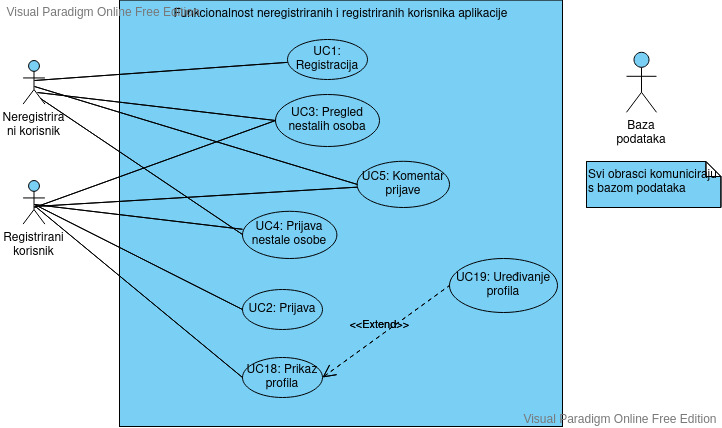
\includegraphics[width=\linewidth]{dijagrami/UML1.vpd.jpg}
					\caption{Dijagram obrasca uporabe, funkcionalnost neregistriranih i registriranih korisnika aplikacije}
	                \end{figure}
	                
				    \begin{figure}[H] 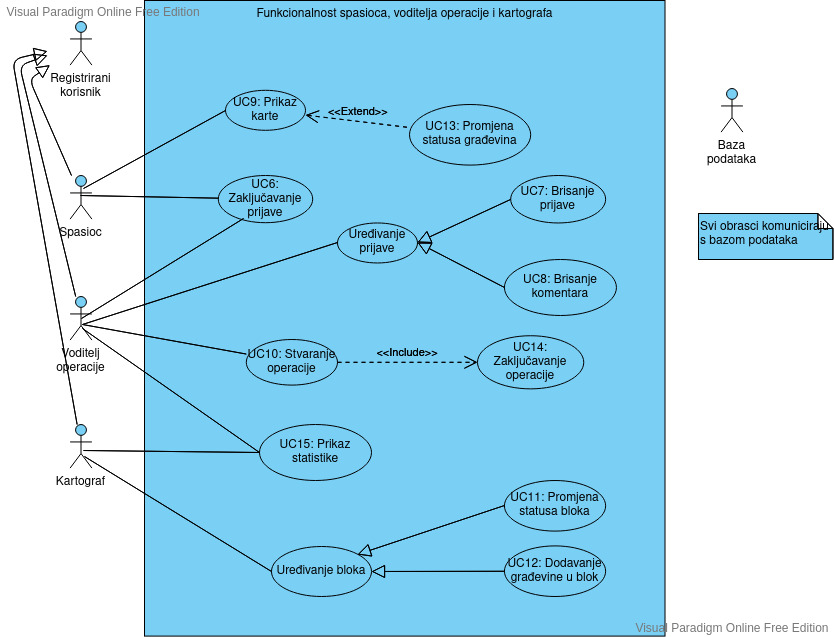
\includegraphics[width=\linewidth]{dijagrami/UML2.vpd.jpg}
				    \caption{Dijagram obrasca uporabe, funkcionalnost spasioca, voditelja operacije i kartografa}
				    \end{figure}
				    
				    \begin{figure}[H] 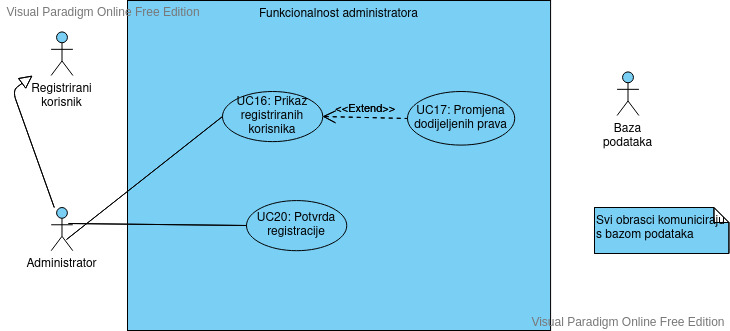
\includegraphics[width=\linewidth]{dijagrami/UML3.vpd.jpg} 
				    \caption{Dijagram obrasca uporabe, funkcionalnost administratora}
				    \end{figure} 
					
				\eject		
				
				\subsection{Sekvencijski dijagrami}
				
				\textbf{Obrazac uporabe UC4 - Prijava nestale osobe}
    
                \textit{Klijent šalje zahtjev za prijavu nestale osobe. Poslužitelj prikazuje obrazac za prijavu. Klijent ispunjava obrazac (ime, prezime, fotografija i opis) za prijavu nestale osobe. Poslužitelj dohvaća podatke iz baze te provjerava je li nova prijavljena osoba u bazi. Ako osoba dosad nije prijavljena, zapisuje se u bazu nestalih te sustav šalje potvrdu i prikaz prijave. Ukoliko je osoba već prijavljena, poslužitelj obavještava klijenta uz poruku.}

                \begin{figure}[H] 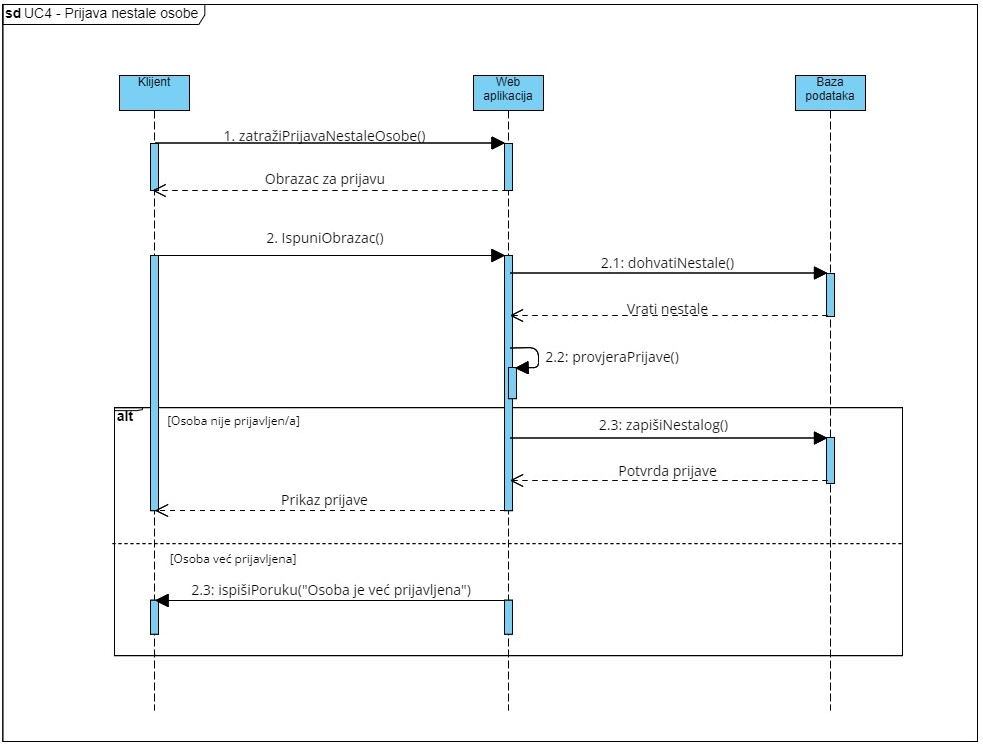
\includegraphics[width=\linewidth]{./dijagrami/PrijavaNestalog.jpg}
				    \caption{Sekvencijski dijagram za UC4 - Prijava nestale osobe}
				    \end{figure}

                \eject

                \textbf{Obrazac uporabe UC10 - Stvaranje operacije}

                \textit{Klijent šalje zahtjev za stvaranje operacije. Sustav provjerava je li korisnik voditelj. Ako korisnik nije voditelj, poslužitelj će ispisati poruku da nema ovlaštenje za stvaranje nove operacije, a ukoliko je, poslat će obrazac za stvaranje nove operacije. Klijent stvara novu operaciju, tj. upisuje ime operacije i područje (regije i blokove) koje je potrebno pretražiti. Poslužitelj dohvaća podatke iz baze te provjerava postoji li već operacija s tim imenom. Ako ne postoji, nova stvorena operacija se zapisuje u bazu podataka te sustav šalje potvrdu i prikaz nove operacije. Ukoliko  već postoji operacija s tim imenom, sustav javlja grešku da je stvorena operacija s već postojećim imenom.}
                
                \begin{figure}[H] 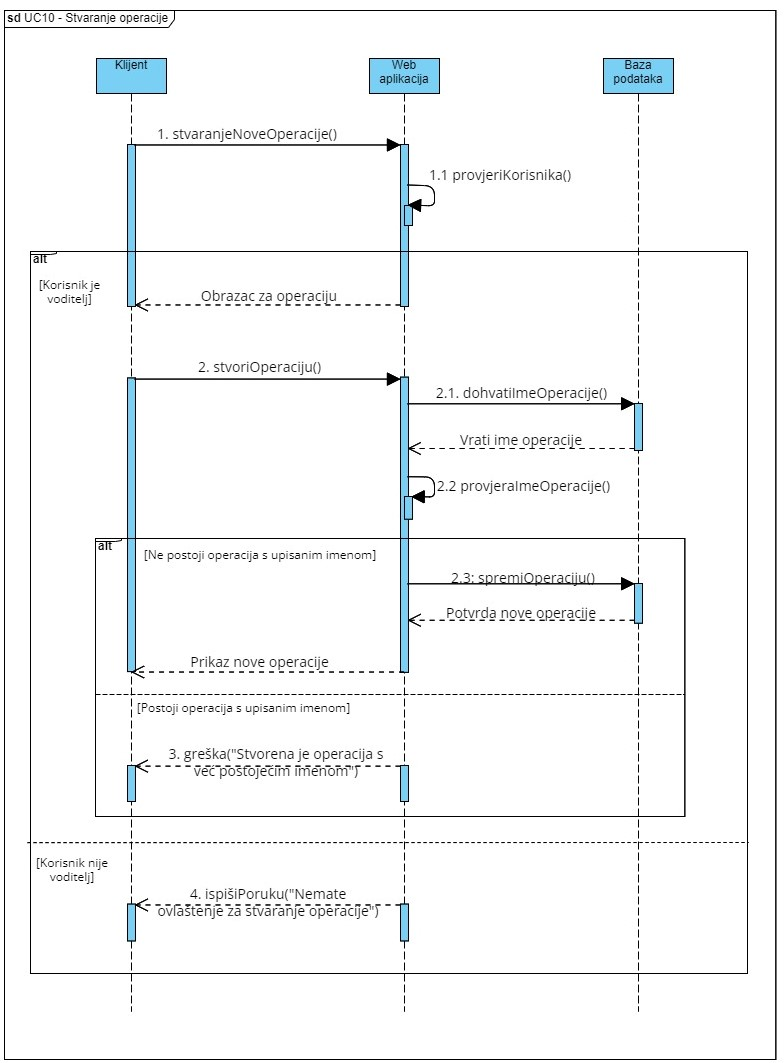
\includegraphics[width=\linewidth]{./dijagrami/StvaranjeOperacije.jpg}
				    \caption{Sekvencijski dijagram za UC10 - Stvaranje operacije}
				    \end{figure}

            	\eject
	
		\section{Ostali zahtjevi}
		
			\textbf{\textit{dio 1. revizije}}\\
		 
			 \textit{Nefunkcionalni zahtjevi i zahtjevi domene primjene dopunjuju funkcionalne zahtjeve. Oni opisuju \textbf{kako se sustav treba ponašati} i koja \textbf{ograničenja} treba poštivati (performanse, korisničko iskustvo, pouzdanost, standardi kvalitete, sigurnost...). Primjeri takvih zahtjeva u Vašem projektu mogu biti: podržani jezici korisničkog sučelja, vrijeme odziva, najveći mogući podržani broj korisnika, podržane web/mobilne platforme, razina zaštite (protokoli komunikacije, kriptiranje...)... Svaki takav zahtjev potrebno je navesti u jednoj ili dvije rečenice.}
			 
			 \begin{itemize}
			 	\item Učitavanje početne stranice, stranice prijave korisnika ili nestalih osoba ne smije trajati duže od nekoliko sekundi
			 	\item Izgled aplikacije treba biti jednostavan kako bi se novi korisnici s lakoćom služili njezinim funkcionalnostima bez dodatnih pomagala (\textit{user-friendly})
			 	\item Proces prijave ili registracije korisnika ne smije trajati duže od nekoliko sekundi
			 	\item Sustav treba podržavati rad i operacije više korisnika u isto vrijeme bez ikakvih poteškoća
			 	\item Operacije vezane uz baze podataka trebaju biti brzo i efikasno izvršene
			 	\item Baza podataka treba biti pouzdana i dobro zaštićena
			 	\item U bazi podataka ne smiju postojati više operacija, korisnika te prijavljenih nestalih osoba s istim imenom
			 	\item Proces prijave nestale osobe ne smije predugo trajati
			 	\item Sustav treba podržavati korištenje dijakritičkih znakova pri unosu imena osoba ili operacija
			 	\item Promjena statusa ili faza blokova u bilo kojem smjeru ne smije narušavati funkcionalnost sustava
			 \end{itemize}
			 
			 
			 
	
